\documentclass[aps, pre, reprint, amsmath, amssymb, superscriptaddress, floatfix]{revtex4-2}

\usepackage{graphicx}
\usepackage{bm}
\usepackage{dcolumn}
\usepackage{hyperref}
\usepackage{xcolor}

\newcommand{\lw}[1]{\textbf{\textcolor{red}{[LW:#1]}}}

\begin{document}

\title{Statistical mechanics of the n-queens lattice gas:\\
Monte Carlo simulations and Poisson mean-field theory}

\author{Zong-Yue Liu}
\affiliation{Department of Physics, Nanjing University, Nanjing 210093, China}

\author{Lei Wang}
\affiliation{Institute of Physics, Chinese Academy of Sciences, Beijing 100190, China}

\date{\today}

\begin{abstract}
We investigate the n-queens problem as a lattice gas---a model in which $N$ queens
are placed on an $N \times N$ chessboard with pairwise repulsive
interactions along shared rows, columns, and diagonals---from the
perspective of statistical mechanics.  The
ground states are exactly the $Q(N)$ solutions of the classical
$N$-queens problem, whose entropy per queen
$s_0 \approx \ln N - \gamma$ ($\gamma \approx 1.942$) exhibits a
characteristic constraint hierarchy: each successive geometric
constraint---columns, then diagonals---reduces the entropy from
the free-placement value $\ln N$ by a definite constant.
We derive the exact high-temperature energy $E/N \to 5/3$ as
$N \to \infty$.
Extensive Monte Carlo simulations with $10^8$ sweeps per temperature
point for $N = 8$--$128$ reveal that the specific heat per queen
$C_v/N$ converges to a universal function of $T$ as $N \to \infty$,
with a non-divergent peak $C_v^{\max}/N \approx 1.62$ at
$T^* \approx 0.237\,J$, establishing the absence of a thermodynamic
phase transition.
Combined with the exactly known high-temperature entropy, the
convergence of $C_v/N$ enables a thermodynamic integration of
$C_v/T$ from $T = \infty$ to $T = 0$ that recovers the ground-state
entropy---and hence the Simkin constant $\gamma$---purely from
Monte Carlo data, providing the first \emph{physical} determination
of this fundamental combinatorial constant.
Supplementary simulations at $N = 256$ and $512$ with a temperature
grid optimized for thermodynamic integration yield
$\gamma_{\rm MC} = 1.94$ at $N = 512$, within $0.1\%$ of the
combinatorial value.
We further construct a Poisson mean-field theory based on independent
attack-line statistics that reproduces the Monte Carlo thermodynamics
to within a few percent, serving as an analytical self-consistency
check.
\end{abstract}

\maketitle

\lw{think about the logic flow of your sections, do they flow well??? 
III and IV does not seem to be in paralel to II and IV}

%=====================================================================
\section{Introduction}
\label{sec:intro}
%=====================================================================

The $N$-queens problem---placing $N$ mutually non-attacking queens on
an $N \times N$ chessboard---is among the oldest combinatorial
problems in mathematics, dating back to the work of Bezzel in
1848~\cite{Bezzel1848}.  Despite its long history, the asymptotic
enumeration of solutions was resolved only recently.  Simkin~\cite{Simkin2022}
proved that the number of solutions $Q(N)$ satisfies
\begin{equation}
  Q(N) = \left((1 \pm o(1))\frac{N}{e^{\gamma}} \right)^N, \quad
  \gamma \approx 1.942,
  \label{eq:QN}
\end{equation}
building on the breakthrough of Bowtell and
Keevash~\cite{Bowtell2023} and earlier bounds by Luria and
Simkin~\cite{Luria2021}.  Nobel, Agrawal, and Boyd~\cite{Nobel2023}
subsequently computed the tightest known bounds on $\gamma$ by
solving Simkin's convex optimization formulation with an
infeasible-start Newton method for board sizes up to $N = 2048$,
narrowing $\gamma$ to the interval
$[1.944\,000\,75,\;1.944\,001\,08]$ \lw{why is is outsize 1.942 ? }
\lw{do you need to list these precise numbers here ? do they matter to your story /}---a precision of ${\sim}\,3
\times 10^{-7}$.  All of these determinations are purely
combinatorial.  Equation~\eqref{eq:QN} yields a ground-state entropy
per queen
$s_0 = \lim_{N \to \infty} \ln Q(N)/N = \ln N - \gamma + o(1)$.

\lw{with unknown o(1) does gamma make sense ?}

Throughout this paper we set $k_B = 1$, so that entropy is
dimensionless and temperature has units of energy.
The form of the ground-state entropy is suggestive.  On an
$N \times N$ lattice, a single particle placed freely in one row has
$\ln N$ units of entropy---the maximal combinatorial freedom per
particle.  The $N$-queens entropy $s_0 = \ln N - \gamma$ can
therefore be read as: each queen retains the full lattice entropy
$\ln N$, reduced by a constant $\gamma$ that encodes the cumulative
cost of geometric constraints.  This constant decomposes naturally
through a hierarchy of constraints with increasing
stringency~\cite{Knuth2022}:
\begin{itemize}
  \item \textit{Free placement} (row constraint only):
    $\Omega = N^N$, $s = \ln N$.
  \item \textit{Permutation} (row + column):
    $\Omega = N!$, $s \approx \ln N - 1$.
  \item \textit{N-queens} (row + column + two diagonals):
    $\Omega \approx (N/e^\gamma)^N$, $s \approx \ln N - \gamma$.
\end{itemize}
The column constraint costs exactly one unit of entropy (the
Stirling correction); the two diagonal constraints together cost
$\gamma - 1 \approx 0.94$ units.  That each geometric constraint
reduces the entropy by a well-defined constant, independent of $N$
in the large-$N$ limit, hints at a deeper statistical-mechanical
structure underlying the combinatorics.

This observation motivates the present work.  We embed the $N$-queens
problem in a lattice gas with tunable
temperature~\cite{Zhang2009,Polson2024} and perform extensive Monte
Carlo simulations. \lw{move your kb = 1 remark here}
 A central finding is that the specific heat per
queen, $C_v/N$, converges to a size-independent curve for
sufficiently large $N$, exhibiting a Schottky-type peak but no phase
transition.  Combined with the exactly known high-temperature entropy
$S(\infty)/N = \frac{1}{N}\ln\binom{N^2}{N} \approx \ln N + 1$,
this convergence enables a thermodynamic integration
\begin{equation*}
  s_0 = \frac{S(\infty)}{N} - \int_0^\infty \frac{C_v}{NT}\,dT,
\end{equation*}
which extracts the ground-state entropy---and hence the Simkin
constant $\gamma$---purely from Monte Carlo simulation data.
This provides the first \emph{physical} route to $\gamma$,
complementary to the combinatorial and optimization-based approaches
that have dominated to date~\cite{Simkin2022,Nobel2023}.  Our thermodynamic extraction yields $\gamma_{\rm MC} = 1.94$ at
$N = 512$ (within $0.1\%$ of the combinatorial value), demonstrating
that a single Monte Carlo campaign can determine a fundamental
combinatorial constant through the laws of thermodynamics.

\lw{why this paragraph ? }
The queen lattice gas also connects to the broader field of
constraint satisfaction problems (CSPs)~\cite{Mezard2009,Krzakala2007}:
the $N$-queens problem sits precisely at the satisfiability threshold
(conflicts become unavoidable for more than $N$ queens), paralleling
random $k$-SAT near its critical clause density.

To gain analytical insight into the thermodynamic curves, we develop a
Poisson mean-field theory based on independent attack-line statistics,
reproducing the energy and specific heat to within a few percent.

The paper is organized as follows.
Section~\ref{sec:model} defines the model.
Section~\ref{sec:entropy} discusses the ground-state entropy.
Section~\ref{sec:highT} derives the exact high-temperature limit.
Section~\ref{sec:mc} presents Monte Carlo results.
Section~\ref{sec:thermo_int} carries out the thermodynamic integration.
Section~\ref{sec:mf} develops the mean-field theory.
Section~\ref{sec:conclusions} concludes.


%=====================================================================
\section{Model and simulation methodology}
\label{sec:model}
%=====================================================================

We consider an $N \times N$ square lattice with open boundary
conditions.  Each site $(i,j)$ ($i,j = 1,\ldots,N$) carries an
occupation variable $n_{ij} \in \{0,1\}$.  The Hamiltonian counts
mutually attacking queen pairs:
\begin{equation}
  H = J \sum_{\langle (i,j),(i',j') \rangle_{\rm attack}}
  n_{ij}\, n_{i'j'},
  \label{eq:H}
\end{equation}
where the sum runs over all pairs sharing a row ($i = i'$), column
($j = j'$), main diagonal ($i - j = i' - j'$), or anti-diagonal
($i + j = i' + j'$), and $J > 0$.  We set $J = 1$ throughout.

The lattice decomposes naturally into \textit{attack lines}: $N$ rows,
$N$ columns, $2N-1$ main diagonals, and $2N-1$ anti-diagonals.
Writing $n_\alpha$ for the number of queens on line $\alpha$, the
Hamiltonian takes the compact form
\begin{equation}
  H = \sum_{\alpha \in \mathcal{L}} \binom{n_\alpha}{2},
  \label{eq:H_lines}
\end{equation}
where $\mathcal{L}$ denotes the set of all $6N - 2$ attack lines and
$\binom{n}{2} = n(n-1)/2$ counts the number of attacking pairs on
each line.  This decomposition into line contributions is the
starting point for both the high-temperature calculation
(Sec.~\ref{sec:highT}) and the mean-field theory (Sec.~\ref{sec:mf}).

We work in the canonical ensemble with fixed particle number
$N$ and use Kawasaki dynamics~\cite{Kawasaki1966}
(queen--vacancy exchange) with the Metropolis acceptance
criterion~\cite{Metropolis1953}.  One \textit{sweep} consists of $N$
attempted exchanges.  Statistical errors are estimated by jackknife
resampling with 200 bins~\cite{Efron1982}.  We simulate $N = 8, 16,
32, 64, 100, 128$ with $10^8$ measurement sweeps per temperature
point (318 temperatures spanning $T = 0.05$ to $400\,J$), preceded by
$2 \times 10^6$ thermalization sweeps, using 32 CPUs in parallel.
We verified ergodicity by running independent simulations from
multiple random initial configurations (seeds); all runs yielded
statistically consistent results for $E/N$ and $C_v/N$ at every
temperature, confirming that the Kawasaki dynamics explores the
configuration space adequately within our thermalization and
measurement windows.

To extend the thermodynamic integration to larger systems, we
performed additional simulations at $N = 256$ and $512$ using a
reduced temperature grid of 126 points optimized for entropy
extraction.  The grid concentrates 80 points in the specific-heat
peak region ($T = 0.105$--$0.500\,J$ in steps of $0.005\,J$) with
$10^8$ measurement sweeps, supplemented by 46 points at lower and
higher temperatures with $10^6$--$10^7$ sweeps.  Since $C_v/N$ has
already converged to its thermodynamic-limit form by $N = 128$
(Sec.~\ref{sec:mc}), these runs are not designed for detailed
finite-size analysis but rather for accurate evaluation of the
integral in Eq.~\eqref{eq:s0_MC}.
The schematic of the model and the relevant length scales are shown in
Fig.~\ref{fig:schematic}.

\begin{figure}[t]
  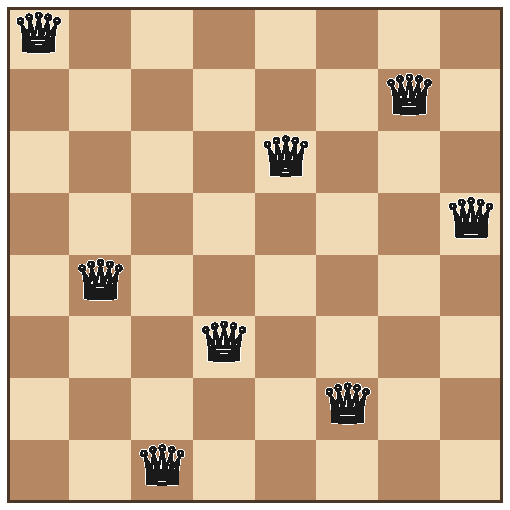
\includegraphics[width=\linewidth]{figures/fig1_schematic.pdf}
  \caption{(a)~A single queen (black circle) on an $8 \times 8$
  board.  Gray squares are attacked along the row, column, and two
  diagonal directions; white squares are unattacked.
  (b)~One of the $Q(8) = 92$ non-attacking ground-state
  configurations.}
  \label{fig:schematic}
\end{figure}


%=====================================================================
\section{Ground-state entropy and constraint hierarchy}
\label{sec:entropy}
%=====================================================================

For $N$ queens, the ground states ($E = 0$) correspond to the
$Q(N)$ non-attacking configurations.  Using
Eq.~\eqref{eq:QN}, the entropy per queen is
\begin{equation}
  s_0 = \frac{\ln Q(N)}{N}
  = \ln N - \gamma + o(1), \quad \gamma \approx 1.942.
  \label{eq:s0}
\end{equation}

The three-level constraint hierarchy (Table~\ref{tab:entropy_levels})
provides a physical interpretation.  Starting from a fully
unconstrained model where each queen independently chooses one of $N$
columns ($\Omega_{\rm free} = N^N$, $s_{\rm free} = \ln N$), the
column non-repetition constraint reduces the count to $N!$
permutations.  By Stirling's approximation,
$\ln N! = N\ln N - N + O(\ln N)$, so the entropy per queen is
\begin{equation}
  s_{\rm perm} = \frac{\ln N!}{N}
  = \ln N - 1 + O\!\left(\frac{\ln N}{N}\right).
  \label{eq:s_perm}
\end{equation}
Thus the column constraint costs exactly one unit of entropy---the
Stirling correction arising from the indistinguishability of column
assignments.

The two diagonal constraints further reduce the entropy to
$s_0 = \ln N - \gamma$, costing an additional $\gamma - 1 \approx
0.94$ units, or approximately $(\gamma - 1)/2 \approx 0.47$ units
per diagonal family.  The hierarchy of costs is physically natural:
the column constraint, being a global permutation on $N$ equivalent
lines, removes exactly one unit of freedom per queen, while each
diagonal family---whose lines have unequal lengths ranging from $1$
to $N$---removes roughly half a unit.

\begin{table}[b]
  \caption{Entropy per queen under successive constraints for the
  $N$-queens problem.  The column constraint costs exactly 1 unit;
  the two diagonal constraints cost $\gamma - 1 \approx 0.94$ units
  combined.}
  \label{tab:entropy_levels}
  \begin{ruledtabular}
  \begin{tabular}{llcc}
    Model & Constraints & $\Omega$ & $s = \frac{1}{N}\ln\Omega$ \\
    \hline
    Free & Row only & $N^N$ & $\ln N$ \\
    Permutation & Row + column & $N!$ & $\ln N - 1$ \\
    $N$-queens & Row + col + 2 diag & $\approx (N/e^\gamma)^N$
      & $\ln N - \gamma$ \\
  \end{tabular}
  \end{ruledtabular}
\end{table}

That each geometric constraint reduces the per-queen entropy by a
constant independent of $N$ suggests that the finite-temperature
thermodynamics may also admit a simple analytical description.  We
turn to this question next, beginning with the high-temperature limit.


%=====================================================================
\section{High-temperature limit}
\label{sec:highT}
%=====================================================================

At $T \to \infty$, all $\binom{N^2}{N}$ configurations with $N$
queens on the $N \times N$ board are equally probable.  We derive the
exact energy using linearity of expectation~\cite{Polson2024}.

Writing the energy as a sum over attack lines
[Eq.~\eqref{eq:H_lines}], each line of length $k$ contributes
$\binom{n}{2} = \frac{1}{2}\sum_{i \ne j} n_i n_j$, where the sum
runs over all pairs of sites on that line.  By linearity of
expectation,
\begin{equation}
  \left\langle\binom{n}{2}\right\rangle
  = \binom{k}{2}\,P(n_i{=}1,\,n_j{=}1).
  \label{eq:line_energy}
\end{equation}
The probability that two given sites are simultaneously occupied is a
combinatorial identity independent of their positions:
\begin{equation}
  P(n_i{=}1,\,n_j{=}1)
  = \frac{\binom{N^2-2}{N-2}}{\binom{N^2}{N}}
  = \frac{N(N-1)}{N^2(N^2-1)}.
  \label{eq:pair_prob}
\end{equation}
The total number of attacking site pairs
$S_{\rm tot} = \sum_\alpha \binom{k_\alpha}{2}$ is obtained by
summing over all attack lines.  Rows contribute
$S_{\rm row} = N\binom{N}{2} = N^2(N{-}1)/2$; columns contribute
identically.  Each diagonal family has $2N{-}1$ diagonals of lengths
$k = N{-}|d|$ ($d = 0, \pm 1, \ldots, \pm(N{-}1)$), giving
\begin{equation}
  S_{\rm diag} = \sum_{d=-(N-1)}^{N-1} \binom{N{-}|d|}{2}
  = \frac{N(N{-}1)(2N{-}1)}{6}
  \label{eq:S_diag}
\end{equation}
per family.  Summing all four families:
\begin{equation}
  S_{\rm tot}
  = 2 \cdot \frac{N^2(N{-}1)}{2}
  + 2 \cdot \frac{N(N{-}1)(2N{-}1)}{6}
  = \frac{N(N{-}1)(5N{-}1)}{3}.
  \label{eq:S_tot}
\end{equation}
Combining Eqs.~\eqref{eq:line_energy}--\eqref{eq:S_tot}, the exact
per-queen energy at $T \to \infty$ is
\begin{equation}
  \frac{\langle E \rangle}{N}\bigg|_{T \to \infty}
  = \frac{S_{\rm tot}}{N} \cdot \frac{N(N-1)}{N^2(N^2-1)}
  = \frac{(5N-1)(N-1)}{3N(N+1)}
  \xrightarrow{N \to \infty} \frac{5}{3}.
  \label{eq:E_highT}
\end{equation}
This result is exact for all finite $N$ and is verified by Monte
Carlo simulations (Fig.~\ref{fig:energy}): at high $T$, $E/N$
converges to the value given by Eq.~\eqref{eq:E_highT}, which
approaches $5/3$ from below with corrections of order $O(1/N)$.


%=====================================================================
\section{Finite-temperature Monte Carlo results}
\label{sec:mc}
%=====================================================================

\subsection{Convergence diagnostics}

Before presenting thermodynamic observables, we verify that the
Monte Carlo simulations have reached equilibrium and that the
measurements are statistically independent.
Figure~\ref{fig:convergence} shows the acceptance rate and the
integrated autocorrelation time $\tau_{\rm int}$ of the energy as
functions of temperature for several system sizes.

The acceptance rate [panel~(a)] increases monotonically with $T$,
reaching $\sim 0.40$--$0.47$ at $T = 1\,J$; it drops below $10^{-5}$
for $T \lesssim 0.1\,J$, reflecting the near-perfect freezing into
non-attacking ground states.  For $N \ge 32$ the curves collapse,
confirming convergence to the thermodynamic limit.

The autocorrelation time [panel~(b)] exhibits a sharp peak at
$T \approx 0.075$--$0.10\,J$, well below the specific heat maximum
$T^* \approx 0.24\,J$, reaching $\tau_{\rm int} \approx 1.8 \times
10^4$ sweeps for $N = 128$.  Even at this worst case, $10^8$
measurement sweeps yield $\sim 5\,500$ independent samples---adequate
for the essentially featureless low-temperature regime where both
$E/N$ and $C_v/N$ approach zero exponentially.  Crucially,
at the physically important specific heat peak ($T \approx 0.225\,J$),
$\tau_{\rm int} \approx 130$--$200$ sweeps for all $N$, providing
more than $5 \times 10^5$ independent samples per temperature point
and ensuring high statistical precision in the region that matters
most.  At $T/J > 0.4$, $\tau_{\rm int}$ falls to $\sim 5$--$10$
sweeps for all system sizes.
We additionally verified ergodicity by comparing independent runs
from different random initial configurations, all yielding
statistically consistent results.

\begin{figure}[t]
  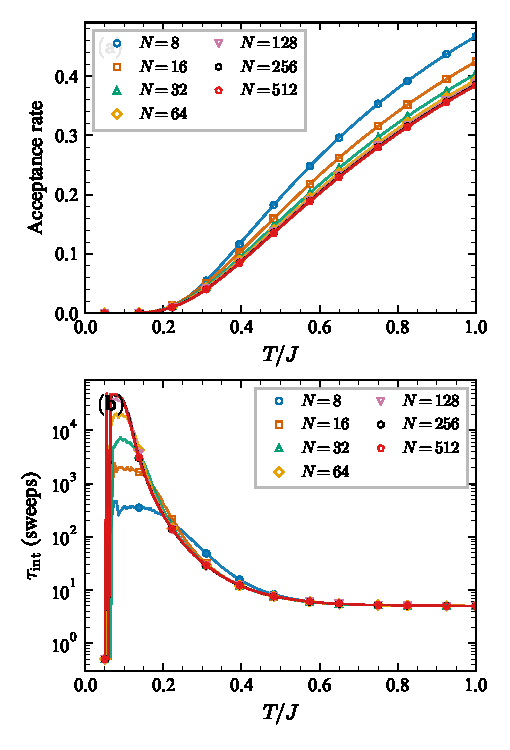
\includegraphics[width=\linewidth]{figures/fig2_convergence.pdf}
  \caption{Convergence diagnostics for the Monte Carlo simulations.
  (a)~Acceptance rate of the Kawasaki (queen--vacancy exchange) moves
  as a function of temperature for $N = 8$--$128$.  The rate drops
  below $10^{-5}$ for $T \lesssim 0.1\,J$ and rises monotonically,
  reaching $0.40$--$0.47$ at $T = 1\,J$.
  (b)~Integrated autocorrelation time $\tau_{\rm int}$ of the energy
  in units of sweeps (log scale).  The sharp peak at
  $T \approx 0.075$--$0.10\,J$ reflects low-temperature freezing and
  lies well below the specific heat maximum $T^* \approx 0.24\,J$;
  at $T^*$ itself, $\tau_{\rm int} \approx 130$--$200$ sweeps,
  yielding more than $5 \times 10^5$ independent samples from $10^8$
  sweeps.}
  \label{fig:convergence}
\end{figure}

\subsection{Energy}

Figure~\ref{fig:energy} shows $E/N$ vs.\ $T$ for $N = 8$--$128$.
The curves for $N \ge 32$ are nearly indistinguishable, confirming
rapid convergence to the thermodynamic limit.
The $N = 256$ and $512$ data (not plotted) are visually
indistinguishable from the $N = 128$ curves at this scale; we omit
them from the figures to preserve the visibility of the convergence
with $N$, and because their coarser temperature grid (126 vs.\ 318
points) and lack of dedicated peak-fitting runs make them less
suitable for detailed $C_v$ peak analysis.  Their role is confined
to the entropy integration of Sec.~\ref{sec:thermo_int}.  At high temperatures,
$E/N$ approaches the exact finite-$N$ value
[Eq.~\eqref{eq:E_highT}], which itself converges to $5/3$ as
$N \to \infty$.

\begin{figure}[t]
  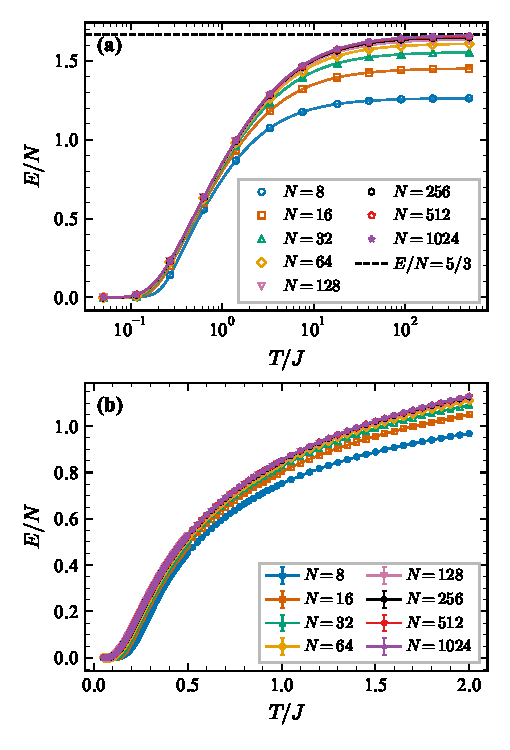
\includegraphics[width=\linewidth]{figures/fig3_energy.pdf}
  \caption{Energy per queen $E/N$ vs.\ temperature for
  $N = 8$--$128$.  (a)~Logarithmic temperature scale over the full
  range $T = 0.05$--$400\,J$; the dashed line marks the analytical
  $N \to \infty$ high-$T$ limit $E/N = 5/3$.  (b)~Linear scale,
  zoomed to $T \le 2\,J$, with error bars.}
  \label{fig:energy}
\end{figure}

\subsection{Specific heat convergence}

The specific heat per queen $C_v/N = (\langle E^2\rangle - \langle
E\rangle^2)/(T^2 N)$ is shown in Fig.~\ref{fig:cv}.  For $N \ge 32$,
the $C_v/N$ curves collapse onto a single function of $T$, indicating
that the thermodynamic limit has been reached.
Table~\ref{tab:cv_peak} lists the peak values.

\begin{figure}[t]
  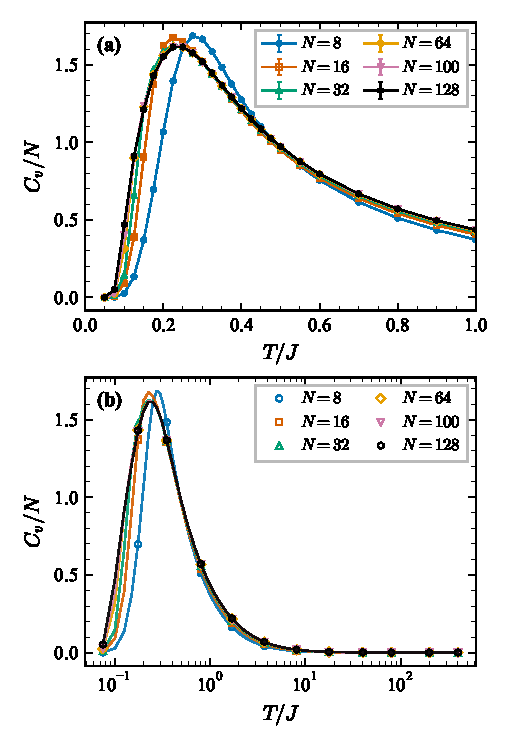
\includegraphics[width=\linewidth]{figures/fig4_cv.pdf}
  \caption{Specific heat per queen $C_v/N$ vs.\ $T$.
  (a)~Peak region ($T \le 1\,J$, linear scale) with error bars.
  (b)~Full temperature range on a logarithmic $T$ scale.
  The curves for $N \ge 32$ collapse onto a single function,
  confirming convergence to the thermodynamic limit.}
  \label{fig:cv}
\end{figure}

\begin{table}[b]
  \caption{$C_v/N$ peak scaling, obtained by
  quartic polynomial fitting with bootstrap resampling (5000 samples).
  The peak height saturates near 1.62 for $N \ge 32$, ruling out a
  divergent susceptibility and hence a continuous phase transition.}
  \label{tab:cv_peak}
  \begin{ruledtabular}
  \begin{tabular}{rD{.}{.}{3}D{.}{.}{4}D{.}{.}{4}}
    $N$ & \multicolumn{1}{c}{$T_{\rm peak}$}
    & \multicolumn{1}{c}{$C_v^{\max}/N$}
    & \multicolumn{1}{c}{error} \\
    \hline
    8   & 0.281 & 1.6915 & 0.0002 \\
    16  & 0.227 & 1.6783 & 0.0006 \\
    32  & 0.231 & 1.6288 & 0.0005 \\
    64  & 0.237 & 1.6216 & 0.0004 \\
    100 & 0.237 & 1.6229 & 0.0004 \\
    128 & 0.237 & 1.6225 & 0.0004 \\
  \end{tabular}
  \end{ruledtabular}
\end{table}

The key observation is that $C_v^{\max}/N$ saturates near $1.62$ for
$N \ge 32$ and does \emph{not} diverge with system size.  This rules
out a thermodynamic phase transition and identifies the crossover as a
Schottky-type anomaly~\cite{Binder2010}---a broad peak in $C_v$
arising from thermal excitation across a finite energy gap, without
any symmetry breaking.  The peak temperature $T^* \approx 0.237\,J$
stabilizes for $N \ge 64$, and the peak height converges
monotonically from above: the residual finite-size correction
between $N = 64$ and $N = 128$ is only $\Delta C_v^{\max}/N
\approx 0.001$, well within the statistical error bars.

The convergence of $C_v/N$ to a definite limiting function has a
powerful consequence: since both the high-temperature entropy
$S(\infty)/N$ and the ground-state entropy $s_0$ are independently
known, the integral $\int_0^\infty C_v/(NT)\,dT$ must equal their
difference.  We exploit this in the next section.


%=====================================================================
\section{Thermodynamic integration and entropy self-consistency}
\label{sec:thermo_int}
%=====================================================================

The convergence of $C_v/N$ to a universal function enables a powerful
thermodynamic self-consistency check.  We compute the entropy
difference between $T = \infty$ and $T = 0$ in two independent ways
and verify that they agree.

\textit{Combinatorial route.}---At $T \to \infty$, all configurations
are equally probable, so the entropy per queen is
\begin{equation}
  \frac{S(\infty)}{N}
  = \frac{1}{N}\ln\binom{N^2}{N}.
  \label{eq:Sinf_def}
\end{equation}
For $N \ll N^2$, applying the Stirling approximation
$\ln n! = n\ln n - n + \tfrac{1}{2}\ln(2\pi n) + O(n^{-1})$:
\begin{align}
  \ln\binom{N^2}{N}
  &= \ln(N^2!) - \ln N! - \ln(N^2 - N)! \notag\\
  &= N\ln N - (N^2{-}N)\ln(1{-}1/N)
  + \Delta_{\rm S},
  \label{eq:Sinf_stirling}
\end{align}
where the first two terms come from the $n\ln n - n$ part of Stirling's
formula and the correction
$\Delta_{\rm S} = \tfrac{1}{2}\ln[N^2/(2\pi N(N^2-N))]
= -\tfrac{1}{2}\ln(2\pi(N-1))$ collects the subleading logarithms.
Expanding $\ln(1 - 1/N) = -1/N - 1/(2N^2) - \cdots$, the
leading terms give $-(N^2-N)\ln(1-1/N) = N - \tfrac{1}{2} + O(N^{-1})$,
so
\begin{equation}
  \frac{S(\infty)}{N}
  = \ln N + 1 + O\!\left(\frac{\ln N}{N}\right).
  \label{eq:Sinf}
\end{equation}
At $T = 0$, only ground states contribute:
$S(0)/N = \ln Q(N)/N \approx \ln N - \gamma$.

\textit{Thermodynamic route.}---The fundamental relation
\begin{equation}
  S(\infty) - S(0) = \int_0^\infty \frac{C_v}{T}\,dT
  \label{eq:thermo_int}
\end{equation}
relates the entropy difference to the specific heat.  Dividing by $N$
and substituting the results above:
\begin{equation}
  \int_0^\infty \frac{C_v}{NT}\,dT
  = \frac{S(\infty) - S(0)}{N}
  = 1 + \gamma + O\!\left(\frac{\ln N}{N}\right).
  \label{eq:DS}
\end{equation}
This is a remarkable relation: the left side involves $C_v(T)$ measured
by simulation over the entire temperature range, while the right side
involves only the \emph{combinatorial} constants 1 (from the Stirling
correction) and $\gamma$ (from the Simkin asymptotic formula).

Rearranging Eq.~\eqref{eq:DS}, we can extract the ground-state
entropy per queen directly from the Monte Carlo data:
\begin{equation}
  s_0^{\rm MC}
  = \frac{S(\infty)}{N} - \int_0^\infty \frac{C_v}{NT}\,dT,
  \label{eq:s0_MC}
\end{equation}
where $S(\infty)/N = \frac{1}{N}\ln\binom{N^2}{N}$ is exact.
This provides a purely thermodynamic determination of the
ground-state degeneracy without direct enumeration.

The numerical integration uses 318 temperature grid points
logarithmically spaced from $T = 0.05\,J$ to $400\,J$; the low-$T$
cutoff contributes negligibly since $C_v/T$ is exponentially
suppressed below $T \approx 0.1\,J$, and the high-$T$ cutoff at
$400\,J$ is sufficient because $C_v/T \propto T^{-3}$ decays
rapidly, contributing less than $0.01\%$ of the integral beyond
this point.  The trapezoidal rule on the logarithmic grid introduces
discretization errors well below the statistical uncertainty of the
Monte Carlo data.

Table~\ref{tab:entropy_check} summarizes the results.
For $N = 8$ and $N = 16$, where exact values of $Q(N)$ are known
($Q(8) = 92$, $Q(16) = 14\,772\,512$), $s_0^{\rm MC}$ agrees with
the exact $s_0^{\rm exact} = \ln Q(N)/N$ to within $1.2\%$ and
$0.5\%$ respectively, validating the simulation and integration
procedure.

For $N \ge 32$, where exact $Q(N)$ is unknown, we use $s_0^{\rm MC}$
to extract the Simkin constant via
$\gamma_{\rm MC} = \ln N - s_0^{\rm MC}$.
The extracted values converge toward the known
asymptotic value $\gamma = 1.942$~\cite{Simkin2022,Nobel2023}:
$\gamma_{\rm MC} = 1.83$ ($N = 32$), $1.89$ ($N = 64$),
$1.90$ ($N = 100$), $1.92$ ($N = 128$, $256$),
and $1.94$ ($N = 512$), with the deviation
decreasing from $5.9\%$ to $0.07\%$ at $N = 512$.
The slight non-monotonicity between $N = 128$ and $N = 256$
($\gamma_{\rm MC} = 1.922$ vs.\ $1.920$) is attributable to the
coarser 126-point temperature grid used for the large-$N$ runs,
which introduces a small discretization error in the numerical
integration comparable to the statistical uncertainty.
The dominant source of error at moderate $N$ is the finite-size
correction to the Simkin formula [the $o(1)$ term in
Eq.~\eqref{eq:QN}], which makes $\gamma_{\rm eff}(N)
= \ln N - s_0(N)$ systematically smaller than the asymptotic
$\gamma$; the MC integration itself introduces only sub-percent
errors, as confirmed by the $N = 8$ and $N = 16$ benchmarks.
The monotonic convergence of $\gamma_{\rm MC}$ toward $1.942$ with
increasing $N$ confirms the mutual consistency of the Monte Carlo
thermodynamics, the Stirling approximation for $S(\infty)$, and the
Simkin combinatorial formula.

\begin{table}[t]
  \caption{Ground-state entropy from thermodynamic integration.
  $s_0^{\rm MC} = S(\infty)/N - \int_0^\infty (C_v/NT)\,dT$, where
  $S(\infty)/N = \frac{1}{N}\ln\binom{N^2}{N}$ is exact.
  For $N \le 16$, $s_0^{\rm MC}$ is compared with the exact
  ground-state entropy $s_0^{\rm exact} = \ln Q(N)/N$.
  For $N \ge 32$, we extract
  $\gamma_{\rm MC} = \ln N - s_0^{\rm MC}$ and compare with the
  Simkin asymptotic value $\gamma = 1.942$.
  The $N = 8$--$128$ data use a 318-point temperature grid;
  $N = 256$ and $512$ use a 126-point grid optimized for the
  entropy integral (see text).}
  \label{tab:entropy_check}
  \begin{ruledtabular}
  \begin{tabular}{cD{.}{.}{3}D{.}{.}{3}D{.}{.}{3}c}
    $N$ & \multicolumn{1}{c}{$s_0^{\rm MC}$}
    & \multicolumn{1}{c}{$s_0^{\rm exact}$}
    & \multicolumn{1}{c}{$\gamma_{\rm MC}$}
    & Deviation \\
    \hline
    8   & 0.558 & 0.565 & \multicolumn{1}{c}{---} & 1.2\% \\
    16  & 1.027 & 1.032 & \multicolumn{1}{c}{---} & 0.5\% \\
    \hline
    32  & 1.639 & \multicolumn{1}{c}{---} & 1.827 & 5.9\% \\
    64  & 2.268 & \multicolumn{1}{c}{---} & 1.891 & 2.6\% \\
    100 & 2.704 & \multicolumn{1}{c}{---} & 1.901 & 2.1\% \\
    128 & 2.931 & \multicolumn{1}{c}{---} & 1.922 & 1.0\% \\
    \hline
    256 & 3.625 & \multicolumn{1}{c}{---} & 1.920 & 1.1\% \\
    512 & 4.298 & \multicolumn{1}{c}{---} & 1.941 & 0.07\% \\
  \end{tabular}
  \end{ruledtabular}
\end{table}


%=====================================================================
\section{Mean-field theory}
\label{sec:mf}
%=====================================================================

The decomposition of $H$ into attack-line contributions
[Eq.~\eqref{eq:H_lines}] suggests a mean-field approach.  We
approximate the occupation numbers on different attack lines as
statistically independent and derive two mean-field theories of
increasing sophistication.

\subsection{Simple Poisson mean-field}

We first present a simple approximation inspired by
Ref.~\cite{Polson2024}.  Each queen interacts along four families of
attack lines (row, column, main diagonal, anti-diagonal), but these
families are not equally constraining: the entropy analysis of
Sec.~\ref{sec:entropy} shows that each row or column constraint
removes one unit of entropy per queen, while the two diagonal
constraints together remove $\gamma - 1 \approx 0.942$ units.
We therefore assign an \emph{entropy-weighted} effective number
of interaction directions,
\begin{equation}
  \nu_{\rm eff} = \underbrace{1 + 1}_{\text{row + column}}
  + \underbrace{(\gamma - 1)}_{\text{two diagonals}} = 1 + \gamma
  \approx 2.942.
  \label{eq:nu_eff}
\end{equation}
Treating each effective direction independently and assigning each
conflict a Boltzmann suppression
$e^{-J/(2T)}$ (the factor of 2 accounts for the pairwise energy being
shared between two queens), the mean-field energy per queen is
\begin{equation}
  \frac{E^{\rm MF}}{N}
  = \frac{(1+\gamma)(N-1)}{2N}\,e^{-1/(2T)}
  \xrightarrow{N \to \infty}
  \frac{1+\gamma}{2}\,e^{-1/(2T)},
  \label{eq:E_simple}
\end{equation}
yielding the specific heat
\begin{equation}
  \frac{C_v^{\rm MF}}{N} = \frac{dE/N}{dT}
  = \frac{1+\gamma}{4T^2}\,e^{-1/(2T)}.
  \label{eq:Cv_simple}
\end{equation}
Setting $dC_v/dT = 0$ gives the peak location $T^* = 1/4$ with
\begin{equation}
  \frac{C_v^{\max}}{N} = \frac{4(1+\gamma)}{e^2} \approx 1.593,
  \label{eq:Cv_peak_simple}
\end{equation}
within $1.8\%$ of the Monte Carlo value $1.623$ for $N = 128$.
We note, however, that this simple MF uses $\gamma$ as an input
parameter [through Eq.~\eqref{eq:nu_eff}], so it cannot serve as an
independent prediction of the thermodynamics---it is inherently
circular if $\gamma$ is the quantity one seeks to determine.

\subsection{Modified Poisson mean-field}

A more systematic---and parameter-free---treatment retains the full
decomposition into four families of attack lines (rows, columns, main
diagonals, anti-diagonals) and accounts for the varying diagonal
lengths, without requiring $\gamma$ as an input.
At finite temperature, the occupation number of a line with mean
$\mu$ (at $T = \infty$) follows the
\textit{modified Poisson distribution}---a Poisson distribution
reweighted by the Boltzmann factor of the intra-line interaction.

For a single attack line with fugacity $\lambda$ at inverse
temperature $\beta = 1/T$, the probability of finding $k$ queens is
\begin{equation}
  P(n = k) = \frac{\lambda^k}{k!}\,
  e^{-\beta\,k(k-1)/2}\Big/\,g(\lambda, \beta),
  \label{eq:modPoisson}
\end{equation}
where the normalizing partition function is
\begin{equation}
  g(\lambda, \beta) = \sum_{k=0}^\infty
  \frac{\lambda^k}{k!}\,e^{-\beta k(k-1)/2}.
  \label{eq:g_def}
\end{equation}
The fugacity $\lambda$ is determined self-consistently by the
constraint $\langle n \rangle = \mu$:
\begin{equation}
  \mu = \frac{\lambda}{g}\,\frac{\partial g}{\partial \lambda}
  = \sum_{k=0}^\infty k\,P(k).
  \label{eq:mu_constraint}
\end{equation}

At $\beta = 0$ ($T \to \infty$), $P(k)$ reduces to a standard Poisson
distribution; at $\beta \to \infty$ ($T \to 0$), only $k = 0$ and
$k = 1$ survive, enforcing the non-attacking constraint.
The expected collision energy per line is
\begin{equation}
  f(\mu, \beta) = \left\langle\binom{n}{2}\right\rangle
  = \frac{1}{2}\sum_{k=2}^{\infty} k(k-1)\,P(k).
  \label{eq:f_def}
\end{equation}

The per-queen energy in the thermodynamic limit is then
\begin{equation}
  \frac{E}{N}(T) = \underbrace{2\,f\!\left(1,\tfrac{1}{T}\right)
  }_{\rm rows + columns}
  + \underbrace{4\int_0^1 f\!\left(\mu,\tfrac{1}{T}\right)d\mu
  }_{\rm diagonals},
  \label{eq:E_MF}
\end{equation}
where the first term sums over $N$ rows and $N$ columns (each with
$\mu = 1$), and the integral accounts for $2 \times (2N-1)$ diagonals
with $\mu = \ell/N \in (0,1]$.

\subsection{Comparison with Monte Carlo}

Figure~\ref{fig:mf} compares both mean-field predictions with Monte
Carlo data ($N = 100$ and $128$).  The modified Poisson MF
systematically overestimates $E/N$ by $2$--$7\%$, an $O(1)$ bias
from the cumulative effect of inter-line correlations.
The simple MF achieves comparable accuracy because the
entropy-weighted prefactor partially absorbs these correlations.
For the specific heat peak, the simple MF gives
$C_v^{\max}/N \approx 1.593$ ($1.8\%$ from MC), while
the modified Poisson MF gives $1.692$ ($4.3\%$ from MC).
Both correctly predict the Schottky shape without any divergence.
Table~\ref{tab:mf_comparison} compares selected temperatures.

\begin{table}[b]
  \caption{Modified Poisson mean-field vs.\ Monte Carlo ($N = 128$).
  The systematic overestimate in $E/N$ is an $O(1)$ effect of
  inter-line correlations neglected by the independent-line
  approximation (see text).}
  \label{tab:mf_comparison}
  \begin{ruledtabular}
  \begin{tabular}{cD{.}{.}{5}D{.}{.}{5}cD{.}{.}{3}D{.}{.}{3}c}
    $T$ & \multicolumn{1}{c}{$E_{\rm MC}/N$}
    & \multicolumn{1}{c}{$E_{\rm MF}/N$}
    & $\Delta E$
    & \multicolumn{1}{c}{$C_{v,\rm MC}/N$}
    & \multicolumn{1}{c}{$C_{v,\rm MF}/N$}
    & $\Delta C_v$ \\
    \hline
    0.200 & 0.12064 & 0.12952 & 7.4\% & 1.554 & 1.646 & 5.9\% \\
    0.225 & 0.16034 & 0.17140 & 6.9\% & 1.615 & 1.692 & 4.8\% \\
    0.300 & 0.27974 & 0.29460 & 5.3\% & 1.520 & 1.550 & 2.0\% \\
    0.500 & 0.52559 & 0.54263 & 3.2\% & 0.973 & 0.976 & 0.3\% \\
    1.000 & 0.84800 & 0.86633 & 2.2\% & 0.436 & 0.439 & 0.7\% \\
  \end{tabular}
  \end{ruledtabular}
\end{table}

\begin{figure}[t]
  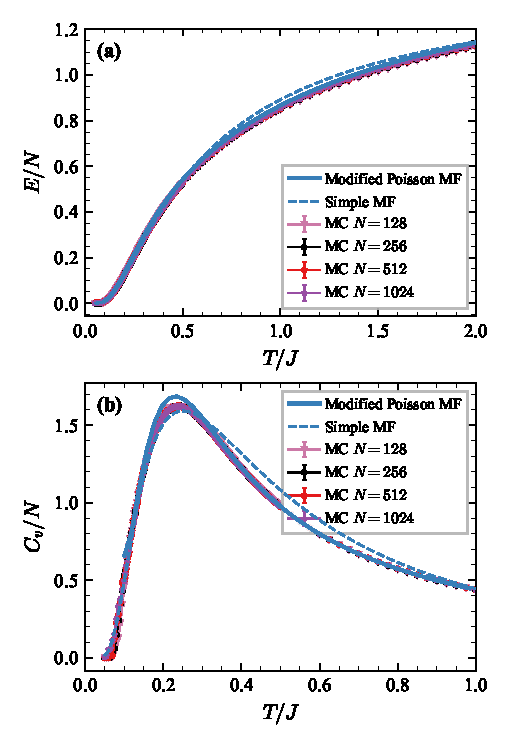
\includegraphics[width=\linewidth]{figures/fig5_meanfield.pdf}
  \caption{Mean-field theory vs.\ Monte Carlo.
  (a)~Energy per queen $E/N$ for $T \le 2\,J$; the solid curve is the
  modified Poisson MF [Eq.~\eqref{eq:E_MF}], the dashed curve is the
  simple MF.  (b)~Specific heat $C_v/N$ for $T \le 1\,J$; both MF
  curves reproduce the peak shape without any divergence.  Only
  $N = 100$ and $N = 128$ MC data are shown, as these are closest to
  the thermodynamic limit.}
  \label{fig:mf}
\end{figure}


%=====================================================================
\section{Conclusions}
\label{sec:conclusions}
%=====================================================================

We have presented a statistical-mechanical investigation of the queen
lattice gas combining extensive Monte Carlo
simulations with analytical mean-field theory.  Our main findings are:

\begin{enumerate}
\item The ground-state entropy $s_0 = \ln N - \gamma$ decomposes
  through a constraint hierarchy: the column constraint costs exactly
  1 unit of entropy per queen (the Stirling correction), while the two
  diagonal constraints together cost $\gamma - 1 \approx 0.94$ units.
  That each constraint reduces the per-queen entropy by an
  $N$-independent constant suggests a statistical-mechanical structure
  amenable to analytical treatment.

\item At $T \to \infty$, the exact energy per queen is
  $E/N = (5N{-}1)(N{-}1)/[3N(N{+}1)] \to 5/3$, derived from a
  linearity-of-expectation argument applied to the uniform random
  placement of queens.

\item The specific heat per queen $C_v/N(T)$ converges to a universal
  function of $T$ as $N \to \infty$.  The peak height $\approx 1.62$
  does not diverge, ruling out a thermodynamic phase transition and
  identifying the crossover as a Schottky anomaly with effective gap
  $\Delta = J$.

\item Thermodynamic integration of $C_v/T$ recovers the ground-state
  entropy per queen $s_0^{\rm MC} = S(\infty)/N - \int(C_v/NT)\,dT$,
  agreeing with exact values at $N = 8$ and $16$ to within $1.2\%$.
  For $N \ge 32$, the extracted Simkin constant
  $\gamma_{\rm MC} = \ln N - s_0^{\rm MC}$ converges
  to $\gamma = 1.942$, reaching $1.94$ at $N = 512$ ($0.07\%$
  deviation).  This nontrivial self-consistency check connects
  the Simkin combinatorial formula, the Stirling approximation for
  the high-temperature entropy, and the Monte Carlo specific heat
  data across the entire temperature range.

\item A modified Poisson mean-field theory, treating each attack line
  as an independent modified Poisson variable, provides an analytical
  expression for $E/N(T)$ and $C_v/N(T)$ that reproduces the Monte
  Carlo data to within $2$--$7\%$.  The simpler entropy-weighted MF
  [$C_v^{\max} = 4(1+\gamma)/e^2$] achieves $1.8\%$ accuracy at the
  peak because its entropy-weighted prefactor partially absorbs
  the correlation effects.

\end{enumerate}

These results establish the queen lattice gas as a model system whose
thermodynamics can be quantitatively described by an independent
attack-line mean-field theory.  The analytical tractability
of the Poisson mean-field approach and the
interplay between combinatorial and thermodynamic quantities make
this model a compelling testbed for ideas at the interface of
constraint satisfaction and statistical mechanics.

A natural next step is to extend the simulations to larger system
sizes ($N \gtrsim 256$), which would yield a more precise
thermodynamic determination of $\gamma$ and further establish the
validity of this physical approach to combinatorial constants.


%=====================================================================
\begin{thebibliography}{30}

\bibitem{Bezzel1848}
M.~Bezzel,
Schachfreund, Berliner Schachzeitung \textbf{3}, 636 (1848).

\bibitem{Simkin2022}
M.~Simkin,
The number of $n$-queens configurations,
Adv.\ Math.\ \textbf{427}, 109127 (2023).

\bibitem{Bowtell2023}
C.~Bowtell and P.~Keevash,
The $n$-queens problem,
arXiv:2109.08083 (2021).

\bibitem{Luria2021}
Z.~Luria and M.~Simkin,
A lower bound for the $n$-queens problem,
arXiv:2105.11431 (2021).

\bibitem{Nobel2023}
P.~Nobel, A.~Agrawal, and S.~Boyd,
Computing tighter bounds on the $n$-queens constant via Newton's
method,
Optim.\ Lett.\ \textbf{17}, 1229 (2023).

\bibitem{Knuth2022}
D.~E.~Knuth,
\textit{The Art of Computer Programming}, Vol.~4B
(Addison-Wesley, 2022), Sec.~7.2.2.

\bibitem{Zhang2009}
C.~Zhang and J.~Ma,
Counting solutions for the $N$-queens and Latin-square problems by
efficient Monte Carlo simulations,
Phys.\ Rev.\ E \textbf{79}, 016703 (2009).

\bibitem{Polson2024}
N.~Polson and V.~Sokolov,
Counting $N$ queens,
arXiv:2407.08830 (2024).

\bibitem{Mezard2009}
M.~M\'ezard and A.~Montanari,
\textit{Information, Physics, and Computation}
(Oxford University Press, Oxford, 2009).

\bibitem{Krzakala2007}
F.~Krzaka{\l}a, A.~Montanari, F.~Ricci-Tersenghi,
G.~Semerjian, and L.~Zdeborov\'a,
Gibbs states and the set of solutions of random constraint
satisfaction problems,
Proc.\ Natl.\ Acad.\ Sci.\ USA \textbf{104}, 10318 (2007).

\bibitem{Kawasaki1966}
K.~Kawasaki,
Diffusion constants near the critical point for time-dependent Ising
models.\ I,
Phys.\ Rev.\ \textbf{145}, 224 (1966).

\bibitem{Metropolis1953}
N.~Metropolis, A.~W.~Rosenbluth, M.~N.~Rosenbluth, A.~H.~Teller,
and E.~Teller,
Equation of state calculations by fast computing machines,
J.~Chem.~Phys.\ \textbf{21}, 1087 (1953).

\bibitem{Efron1982}
B.~Efron,
\textit{The Jackknife, the Bootstrap, and Other Resampling Plans}
(SIAM, Philadelphia, 1982).

\bibitem{Binder2010}
K.~Binder and D.~W.~Heermann,
\textit{Monte Carlo Simulation in Statistical Physics}
(Springer, Berlin, 5th ed., 2010).

\end{thebibliography}

\end{document}
